\documentclass[border=5pt]{standalone}
\usepackage{tikz}
\usepackage{amssymb}
\usepackage{xcolor}

\usetikzlibrary{shapes,positioning,backgrounds,fit,intersections}

% Define colors
\definecolor{leftcircle}{RGB}{192,224,255} % Light blue
\definecolor{rightcircle}{RGB}{255,192,203} % Light pink/orange
\definecolor{intersection}{RGB}{153,102,255} % Purple
\definecolor{broadtext}{RGB}{153,204,255} % Light blue

\begin{document}
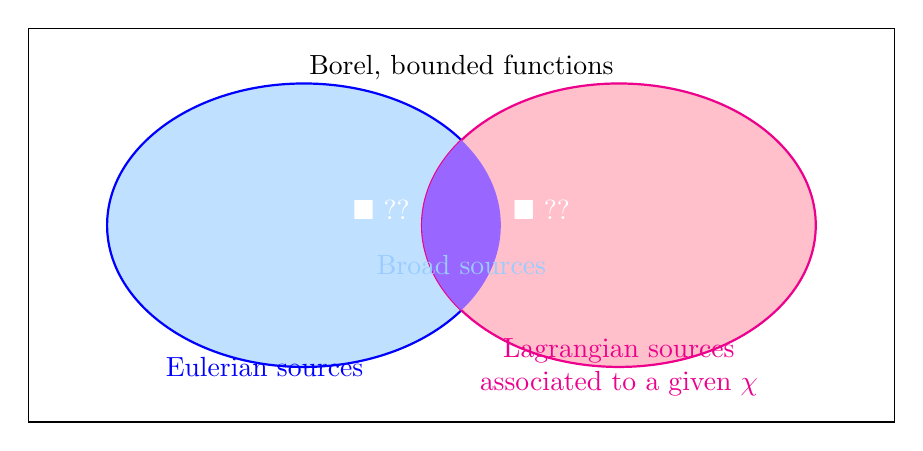
\begin{tikzpicture}[
  scale=1.0,
  every node/.style={font=\normalsize},
]

% Draw external rectangle frame
\draw[black, line width=0.5pt] (-5.5,-2.5) rectangle (5.5,2.5);

% Title
\node at (0,2) {Borel, bounded functions};

% Left ellipse (Eulerian sources)
\fill[leftcircle] (-2,0) ellipse (2.5cm and 1.8cm);
\draw[draw=blue, line width=0.8pt] (-2,0) ellipse (2.5cm and 1.8cm);
\node[text=blue, align=center] at (-2.5,-1.8) {Eulerian sources};

% Right ellipse (Lagrangian sources)
\fill[rightcircle] (2,0) ellipse (2.5cm and 1.8cm);
\draw[draw=magenta, line width=0.8pt] (2,0) ellipse (2.5cm and 1.8cm);
\node[text=magenta, align=center] at (2,-1.8) {Lagrangian sources\\associated to a given $\chi$};

% Intersection region
\begin{scope}
  \clip (-2,0) ellipse (2.5cm and 1.8cm);
  \fill[intersection] (2,0) ellipse (2.5cm and 1.8cm);
\end{scope}

% Question marks
\node[text=white] at (0,0.2) {$\blacksquare$ ?? \hspace{1cm} $\blacksquare$ ??};

% "Broad sources" label
\node[text=broadtext] at (0,-0.5) {Broad sources};

\end{tikzpicture}
\end{document}